\section{Other techniques and performance gain}


We used the EPCC microbenchmarks\cite{Bul99} to show the performance
gains coming from optimization considerations we discussed in previous
sections. The hardware systems we tested on are a 16-way 375MHz
POWER3$^{TM}$ and a 32-way 1.1GHz POWER4$^{TM}$.

The EPCC benchmarks have two parts, the synchronization suite and the
schedule suite. Since we are concentrating on workshare
implementation, we have focused on the synchronization benchmark. It
includes separate test cases for parallel region, workshares (which are
OMP DO, SINGLE and explicit barrier), and reductions.

For a parallel region, as we show in Figure \ref{fig:compare}, the ``on
demand'' initialization method introduced in section
\ref{sec:optimize} reduces its overhead on both POWER3 and POWER4
systems. 

%This is the actual improvement we had over XL Fortran 8.1 and C/C++
%6.0.

\begin{figure}[!h]
  \begin{center}
    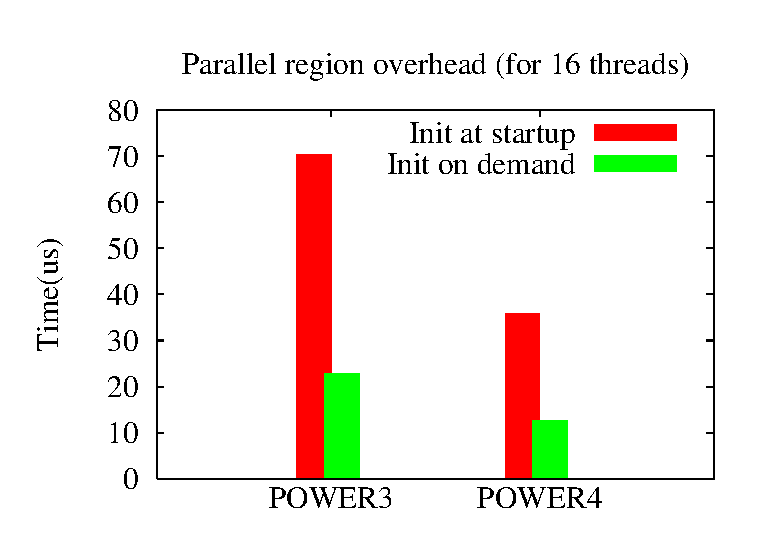
\includegraphics[angle=0, width=0.60\textwidth]{compare.eps}
    \caption{\footnotesize Performance difference}
    \label{fig:compare}
  \end{center}
\end{figure}

For a barrier operation, we compare a primitive fetch-and-add barrier
with the one using algorithm \ref{alg:barrier} and the results are
shown in Figure \ref{fig:power4performance}. The test was done on the
POWER4 system. As the number of threads increases, the advantage of
using distributed counters becomes more apparent.

\begin{figure}[!h]
  \begin{center}
    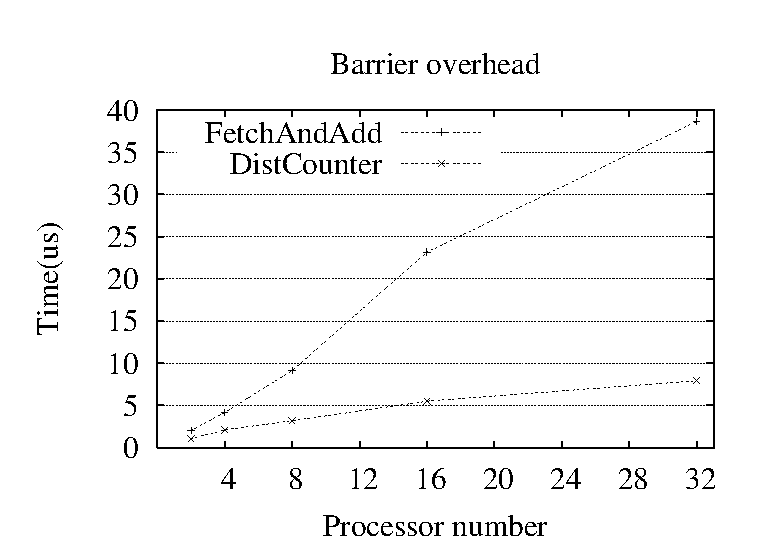
\includegraphics[angle=0, width=0.60\textwidth]{power4performance.eps}
    \caption{\footnotesize POWER4 barrier overhead}
    \label{fig:power4performance}
  \end{center}
\end{figure}

In fact, the whole sub-suite improved significantly with the methods
introduced in the previous sections. Again the data in Figure
\ref{fig:epcc} was collected on the POWER4 system.

\begin{figure}[!h]
  \begin{center}
    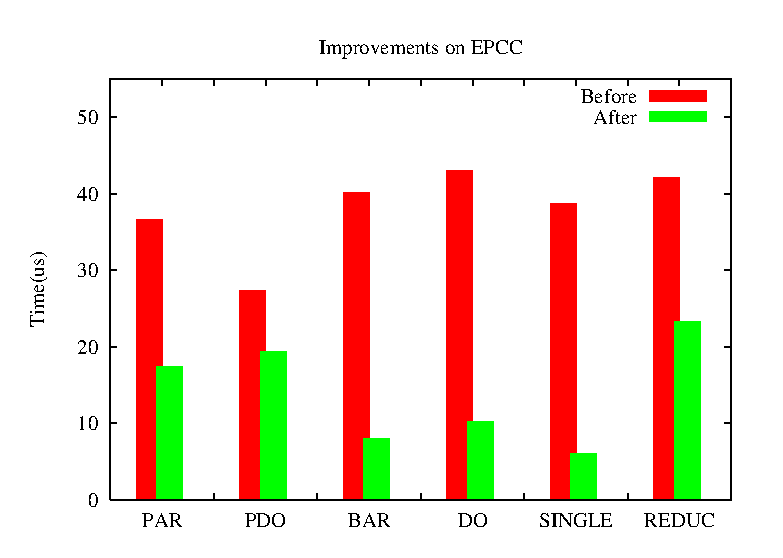
\includegraphics[angle=0, width=0.80\textwidth]{epcc.eps}
    \caption{\footnotesize EPCC improvement}
    \label{fig:epcc}
  \end{center}
\end{figure}

Note that in this figure, the reduction case is special; aside from
the improvement from a better parallel region and synchronization
method, we have also implemented a partial-sum mechanism to implement
the reduction, which allows us to minimize the required
synchronization.

% Both tests uses 16 threads.

%{\small
%\begin{verbatim}
%      dl = delaylength

%      do k=0,outerreps
%         start  = getclock()
%         do j=1,innerreps
%!$OMP PARALLEL
%            call delay(dl)
%!$OMP END PARALLEL
%         end do
%         time(k) = (getclock() - start) * 
%     &       1.0e6 / dble (innerreps)
%      end do
%\end{verbatim}
%}

%\emph{[More to be added, including complete EPCC results and analysis ... ]}

